\qrchapter{https://forgottenpillar.com/rsc/en-fp-chapter1}{The historical context}


\qrchapter{https://forgottenpillar.com/rsc/en-fp-chapter1}{Muktadha wa kihistoria}


Ellen White recalled encountering the same sentiments in \textit{The Living Temple} that she had warned against early in her ministry:


Ellen White alikumbuka kukutana na maoni yale yale katika \textit{The Living Temple} ambayo alikuwa ameonywa dhidi yake mapema katika huduma yake:


\egw{As we read \normaltext{[The Living Temple]}, I recognized the very sentiments against which I had been bidden to speak in warning \textbf{during the early days of my public labors}. \textbf{When I first left \underline{the State of Maine, it was to go through Vermont and Massachusetts}}, to bear a testimony \textbf{against these sentiments}. ‘Living Temple’ contains the alpha of these theories. I knew that the omega would follow in a little while; and I trembled for our people. I knew that I must warn our brethren and sisters \textbf{not to enter into controversy over \underline{the presence and personality of God}}. The statements made in ‘Living Temple’ in regard to this point are incorrect. The scripture used to substantiate the doctrine there set forth, is scripture misapplied.}[SpTB02 53.2; 1904][https://egwwritings.org/read?panels=p417.271]


\egw{Tulipokuwa tunasoma \normaltext{[The Living Temple]}, nilitambua maoni yale yale ambayo nilikuwa nimeamriwa kuyaongea kwa onyo \textbf{wakati wa siku za mwanzo za kazi yangu ya hadhara}. \textbf{Nilipotoka kwanza \underline{Jimbo la Maine, ilikuwa ni kupitia Vermont na Massachusetts}}, kubeba ushuhuda \textbf{dhidi ya maoni haya}. ‘Living Temple’ ina alfa ya nadharia hizi. Nilijua kwamba omega ingefuata baada ya muda mfupi; na nilitetemeka kwa ajili ya watu wetu. Nilijua kwamba nilihitaji kuwaonya ndugu na dada zetu \textbf{wasijihusishe na mgogoro juu ya \underline{uwepo na umbile la Mungu}}. Taarifa zilizotolewa katika ‘Living Temple’ kuhusiana na nukta hii si sahihi. Maandiko yaliyotumika kuthibitisha mafundisho yaliyowekwa hapo, ni maandiko yaliyotumika vibaya.}[SpTB02 53.2; 1904][https://egwwritings.org/read?panels=p417.271]


She pinpointed her first encounter with these views: \egwinline{When I first left \textbf{the State of Maine}, it was to go through Vermont and Massachusetts, \textbf{to bear a testimony against these sentiments.}} Her biography, written by her grandson Arthur Lacey White, provides further context on these sentiments. In \textit{Ellen White: The Early Years}, under the section \textit{Wrestling with the Views of the Spiritualizers}, her experiences in eastern Maine reveal more about the controversy over the personality of God and its implications.


Alitaja kukutana kwake kwa mara ya kwanza na maoni haya: \egwinline{Nilipotoka kwanza \textbf{Jimbo la Maine}, ilikuwa ni kupitia Vermont na Massachusetts, \textbf{kubeba ushuhuda dhidi ya maoni haya.}} Wasifu wake, ulioandikwa na mjukuu wake Arthur Lacey White, unatoa muktadha zaidi kuhusu maoni haya. Katika \textit{Ellen White: The Early Years}, chini ya sehemu \textit{Wrestling with the Views of the Spiritualizers}, uzoefu wake katika mashariki ya Maine unafunua zaidi kuhusu mgogoro juu ya umbile la Mungu na maana zake.


\othersQuote{\textbf{\underline{In eastern Maine} Ellen was traveling} and working \textbf{in the atmosphere of the spiritualizers who had \underline{allegorized away heaven, God, Jesus, and the Advent hope}}. In the vision at Exeter in mid-February she seemed to be \textbf{in the presence of Jesus, and she was eager to procure answers to some \underline{vital questions}}.}[ALW, 1BIO 79.4; 1985][https://egwwritings.org/read?panels=p668.582]


\othersQuote{\textbf{\underline{Katika mashariki ya Maine} Ellen alikuwa akisafiri} na kufanya kazi \textbf{katika mazingira ya wale wanaofanya mambo ya kiroho ambao walikuwa \underline{wamefanya mbingu, Mungu, Yesu, na tumaini la Ujio kuwa mafumbo}}. Katika maono huko Exeter katikati ya Februari alionekana \textbf{kuwa katika uwepo wa Yesu, na alikuwa na hamu ya kupata majibu ya baadhi ya \underline{maswali muhimu}}.}[ALW, 1BIO 79.4; 1985][https://egwwritings.org/read?panels=p668.582]


\othersQuoteNoGap{I asked Jesus if \textbf{His Father had a form like Himself}. \textbf{He said He had}, but I could not behold it, for said He, ‘If you should once behold the glory of \textbf{His person}, you would cease to exist.’—Early Writings, 54.}[ALW, 1BIO 79.5; 1985][https://egwwritings.org/read?panels=p668.583]


\othersQuoteNoGap{Nilimwuliza Yesu kama \textbf{Baba yake alikuwa na umbo kama Yeye}. \textbf{Akasema alikuwa nalo}, lakini sikuweza kuliona, kwani alisema, ‘Kama ungaliona mara moja utukufu wa \textbf{Umbile Lake}, ungekoma kuwepo.’—Early Writings, 54.}[ALW, 1BIO 79.5; 1985][https://egwwritings.org/read?panels=p668.583]


\othersQuoteNoGap{This was not the only occasion Ellen was to converse with Jesus and the angel \textbf{about the \underline{person of Jesus} and concerning \underline{God being a personal being}}. \textbf{\underline{The answers satisfied her fully that the spiritualizers were in gross error}}.}[ALW, 1BIO 80.1; 1985][https://egwwritings.org/read?panels=p668.586]


\othersQuoteNoGap{Hii haikuwa tukio la pekee ambapo Ellen aliongea na Yesu na malaika \textbf{kuhusu \underline{nafsi ya Yesu} na kuhusu \underline{Mungu kuwa nafsi binafsi}}. \textbf{\underline{Majibu yalimridhisha kabisa kwamba wale wanaofanya mambo ya kiroho walikuwa katika makosa makubwa}}.}[ALW, 1BIO 80.1; 1985][https://egwwritings.org/read?panels=p668.586]


The vision Arthur Lacey White referred to is known as the \textit{vision on the personality of God}, which we will examine later. This vision confirms that the doctrine of the \emcap{personality of God} teaches that God the Father has a form, just as Jesus does. It specifically addresses the \others{\textbf{person of Jesus} and concerning \textbf{God being a personal being}.}


Maono ambayo Arthur Lacey White aliyarejea yanajulikana kama \textit{maono juu ya umbile la Mungu}, ambayo tutayachunguza baadaye. Maono haya yanathibitisha kwamba fundisho la \emcap{umbile la Mungu} linafundisha kwamba Mungu Baba ana umbo, kama vile Yesu alivyo. Inaelezea hasa kuhusu \others{\textbf{nafsi ya Yesu} na kuhusu \textbf{Mungu kuwa nafsi binafsi}.}


\begin{figure}[t]
    \centering
    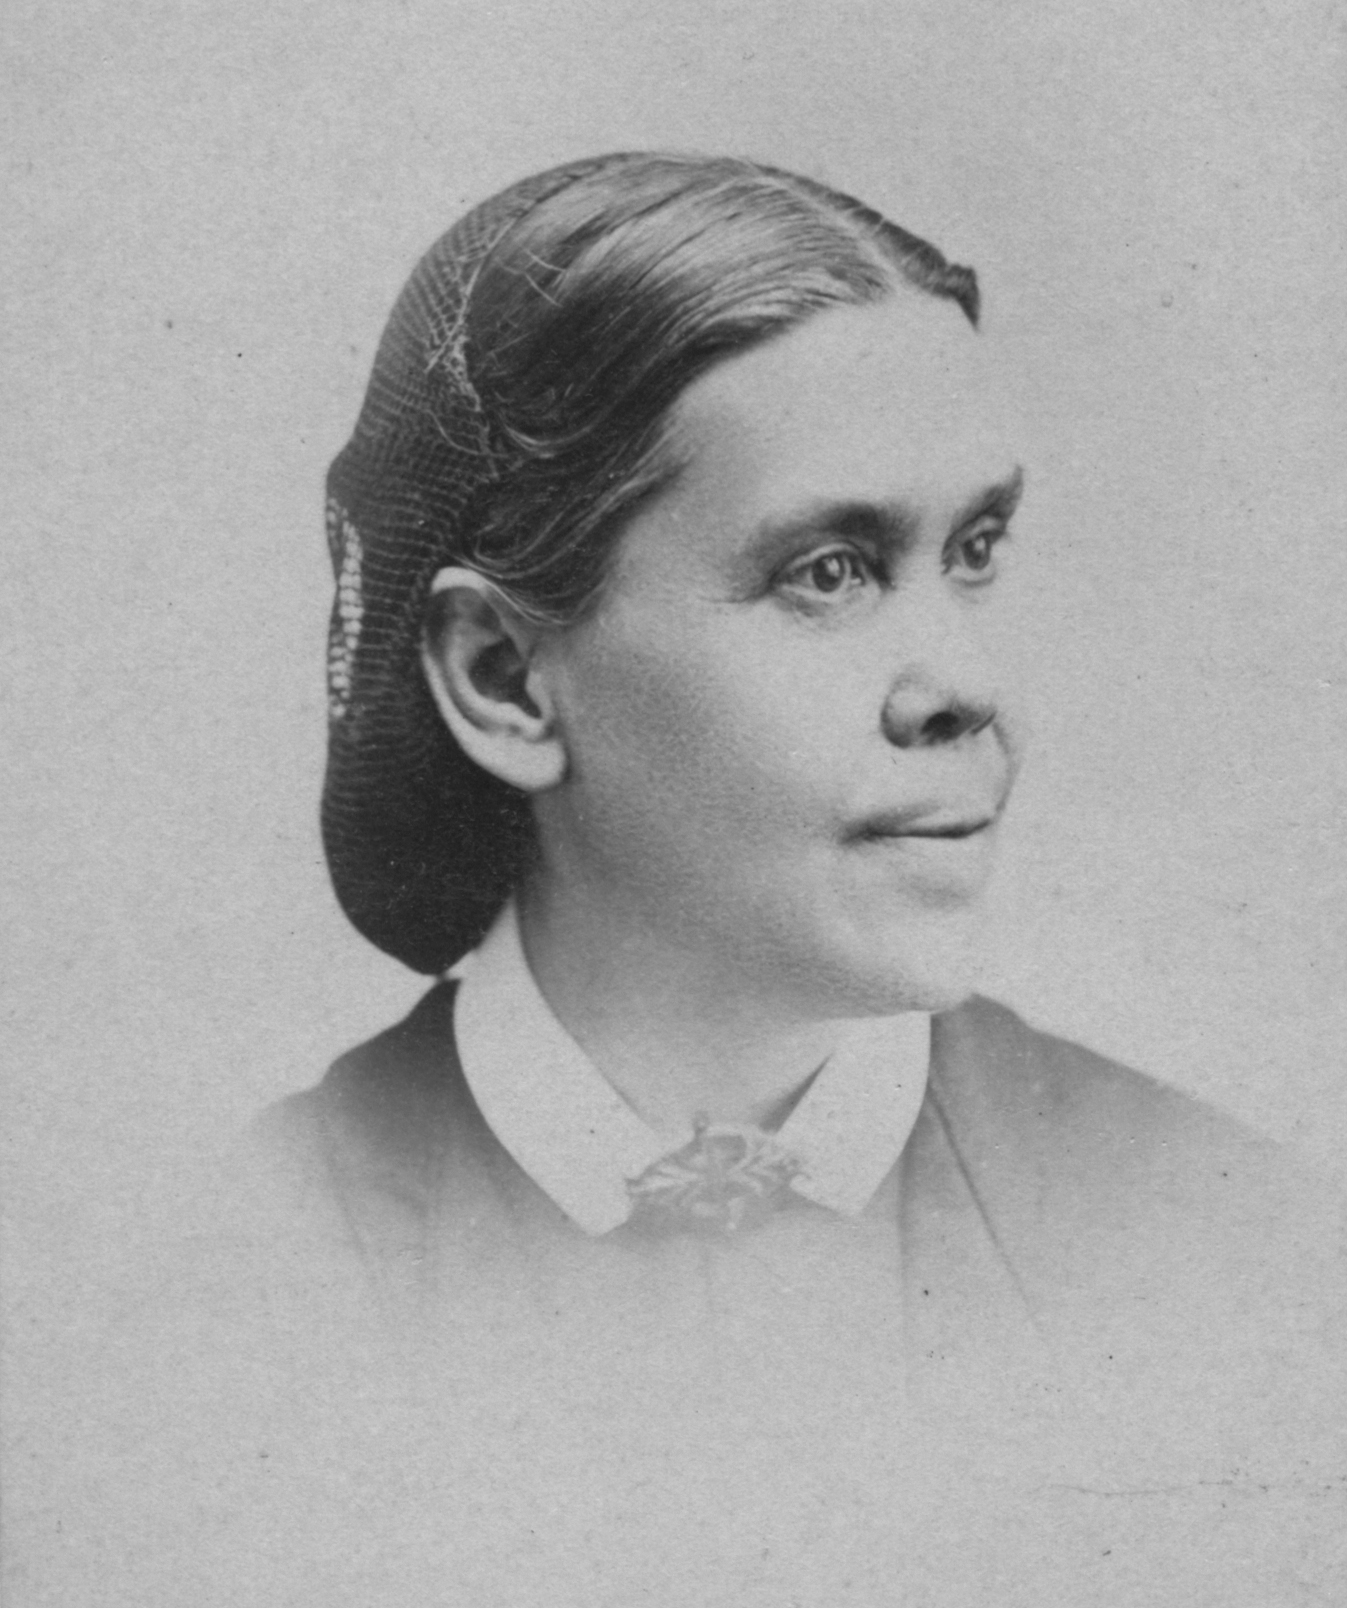
\includegraphics[width=0.65\linewidth]{images/ellen-white.jpg}
    \caption*{Ellen G. White}
    \label{fig:ellen-g-white}
\end{figure}


\begin{figure}[t]
    \centering
    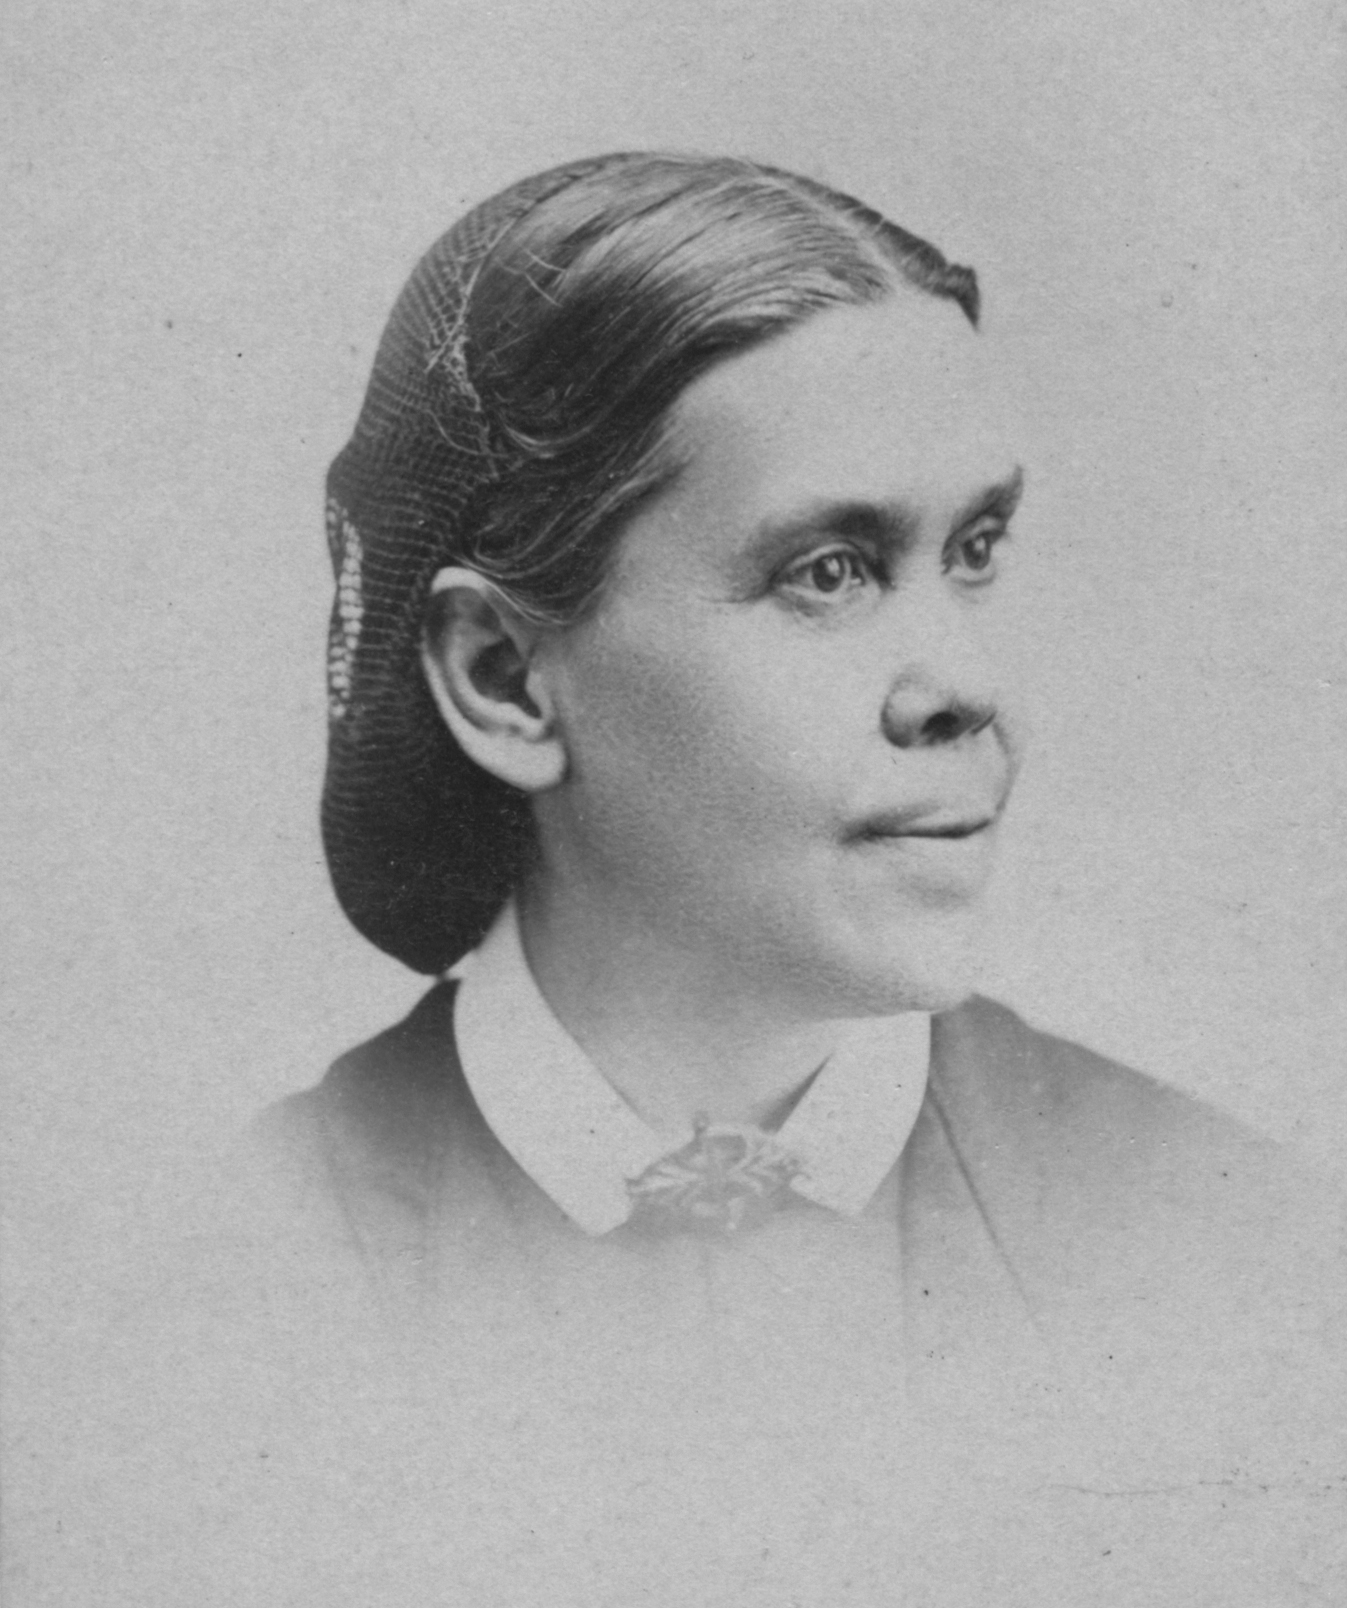
\includegraphics[width=0.65\linewidth]{images/ellen-white.jpg}
    \caption*{Ellen G. White}
    \label{fig:ellen-g-white}
\end{figure}


Consider the first point of the \emcap{Fundamental Principles}, which states that Seventh-day Adventists believe in \others{one God, \textbf{a personal, spiritual being}.}[First point of the Fundamental Principles][https://forgotten-pillar.s3.us-east-2.amazonaws.com/A+declaration+of+the+fundamental+principles+taught+and+practiced+by+the+Seventh-day+Adventists++.pdf] This makes it clear that the central issue in the doctrine of the \emcap{personality of God} concerns the outward, bodily form of the Father. But why was this such a vital and significant question? What were the implications of God having a bodily, personal form?


Fikiria nukta ya kwanza ya \emcap{Kanuni za Kimsingi}, ambayo inasema kwamba Waadventista Wasabato wanaamini katika \others{Mungu mmoja, \textbf{nafsi binafsi, kiumbe cha kiroho}.}[First point of the Fundamental Principles][https://forgotten-pillar.s3.us-east-2.amazonaws.com/A+declaration+of+the+fundamental+principles+taught+and+practiced+by+the+Seventh-day+Adventists++.pdf] Hii inafanya iwe wazi kwamba suala kuu katika fundisho la \emcap{umbile la Mungu} linahusu umbo la nje, la kimwili la Baba. Lakini kwa nini hili lilikuwa swali muhimu na la maana sana? Nini maana ya Mungu kuwa na umbo la kimwili, la kibinafsi?


\othersQuote{But because the pioneers of the Seventh-day Adventist Church held that prophecy was fulfilled on October 22, 1844, and that an important work began in heaven in the Most Holy Place of the heavenly sanctuary at that time, and because the Adventists who had become \textbf{spiritualizers} took the position that Christ had come into their hearts on October 22, 1844, and that His kingdom was in their hearts, the founders of the church, and notably Ellen White, were classed by the world generally, and also by those that SDAs have termed first-day Adventists, as one and the same group. Here again the great enemy cast aspersion upon the true, paralleling it with a false, spurious experience.}[ALW, 1BIO 80.2; 1985][https://egwwritings.org/read?panels=p668.587]


\othersQuote{Lakini kwa sababu waanzilishi wa Kanisa la Waadventista Wasabato walishikilia kwamba unabii ulitimizwa Oktoba 22, 1844, na kwamba kazi muhimu ilianza mbinguni katika Patakatifu pa Patakatifu pa hekalu la mbinguni wakati huo, na kwa sababu Waadventista ambao walikuwa wamekuwa \textbf{wanarohanishaji} walichukua msimamo kwamba Kristo alikuwa amekuja ndani ya mioyo yao Oktoba 22, 1844, na kwamba Ufalme wake ulikuwa ndani ya mioyo yao, waanzilishi wa kanisa, na hasa Ellen White, waliwekwa na ulimwengu kwa ujumla, na pia na wale ambao Waadventista Wasabato wamewataja kama Waadventista wa siku ya kwanza, kama kundi moja na lilelile. Hapa tena adui mkuu alitupa shutuma juu ya ukweli, akilinganisha na uzoefu wa uongo, bandia.}[ALW, 1BIO 80.2; 1985][https://egwwritings.org/read?panels=p668.587]


\othersQuoteNoGap{Ellen White was to speak of this matter again, particularly in the closing paragraphs of her first little book, Experience and Views, published in 1851. As one reads this he will note the use of \textbf{the term spiritualism}, which must be taken in the light of the work of the spiritualizers and not in the light of what today is understood to be spiritualism or spiritism, although both emanate from the same source.}[ALW, 1BIO 80.3; 1985][https://egwwritings.org/read?panels=p668.588]


\othersQuoteNoGap{Ellen White alikuwa azungumzie jambo hili tena, hasa katika aya za mwisho za kitabu chake cha kwanza kidogo, Experience and Views, kilichochapishwa mwaka 1851. Mtu anapoisoma hii ataona matumizi ya \textbf{neno uchawi}, ambalo lazima lichukuliwe katika mwanga wa kazi ya wanarohanishaji na sio katika mwanga wa kile ambacho leo kinafahamika kuwa uchawi au ushetani, ingawa vyote vinatoka kwenye chanzo kilekile.}[ALW, 1BIO 80.3; 1985][https://egwwritings.org/read?panels=p668.588]


\othersQuoteNoGap{We turn now to the statement written and published in 1851 as found in Ibid., 77, 78:}[ALW, 1BIO 80.4; 1985][https://egwwritings.org/read?panels=p668.589]


\othersQuoteNoGap{Sasa tunageukia taarifa iliyoandikwa na kuchapishwa mwaka 1851 kama inavyopatikana katika Ibid., 77, 78:}[ALW, 1BIO 80.4; 1985][https://egwwritings.org/read?panels=p668.589]


\othersQuoteNoGap{\textbf{I have frequently been falsely charged with teaching views peculiar to Spiritualism}. But before the editor of The Day-Star ran into that delusion, \textbf{the Lord \underline{gave me a view} of the sad and desolating effects that would be produced upon the flock by him and others \underline{in teaching the spiritual views}}.}[ALW, 1BIO 80.5; 1985][https://egwwritings.org/read?panels=p668.590]


\othersQuoteNoGap{\textbf{Mara nyingi nimeshtakiwa kwa uongo kwa kufundisha maoni yanayofanana na Uchawi}. Lakini kabla mhariri wa The Day-Star hajaingia katika upotovu huo, \textbf{Bwana \underline{alinipa maono} ya matokeo ya kusikitisha na ya kuharibu ambayo yangezalishwa juu ya kundi na yeye na wengine \underline{katika kufundisha maoni ya kiroho}}.}[ALW, 1BIO 80.5; 1985][https://egwwritings.org/read?panels=p668.590]


\othersQuoteNoGap{I have often seen the lovely \textbf{Jesus, that He is a person}. I asked Him \textbf{\underline{if His Father was a person} and \underline{had a form} like Himself}. Said Jesus, ‘I am in \textbf{the express image of My Father’s person}.}[ALW, 1BIO 80.6; 1985][https://egwwritings.org/read?panels=p668.591]


\othersQuoteNoGap{Mara nyingi nimemwona \textbf{Yesu mzuri, kwamba Yeye ni Nafsi}. Nilimwuliza \textbf{\underline{kama Baba yake alikuwa Nafsi} na \underline{alikuwa na umbo} kama Yeye}. Yesu alisema, ‘Mimi ni \textbf{chapa kamili ya Umbile Wake}.}[ALW, 1BIO 80.6; 1985][https://egwwritings.org/read?panels=p668.591]


\othersQuoteNoGap{\textbf{I have often seen that \underline{the spiritual view} took away all the glory of heaven, and that in many minds the throne of David and the lovely person of Jesus have been burned up in the fire of Spiritualism.} I have seen that some who have been deceived and led into this error will be brought out into the light of truth, but it will be almost impossible for them to get entirely rid of \textbf{the deceptive power of Spiritualism}. Such should make thorough work in confessing their errors and leaving them forever.}[ALW, 1BIO 80.7; 1985][https://egwwritings.org/read?panels=p668.592]


\othersQuoteNoGap{\textbf{Mara nyingi nimeona kwamba \underline{mtazamo wa kiroho} uliondoa utukufu wote wa mbinguni, na kwamba katika akili nyingi kiti cha enzi cha Daudi na nafsi nzuri ya Yesu zimeteketezwa katika moto wa Uchawi.} Nimeona kwamba baadhi ya wale ambao wamedanganywa na kuongozwa katika kosa hili wataleta nje katika nuru ya ukweli, lakini itakuwa karibu haiwezekani kwao kuondokana kabisa na \textbf{nguvu ya udanganyifu wa Uchawi}. Watu kama hao wanapaswa kufanya kazi ya kina katika kukiri makosa yao na kuyaacha milele.}[ALW, 1BIO 80.7; 1985][https://egwwritings.org/read?panels=p668.592]


\othersQuoteNoGap{\textbf{The spiritualization of heaven, God, Christ, and the coming of Christ lay at the foundation of much of the fanatical teachings that 17-year-old Ellen Harmon was called upon by God to meet in those formative days. The visions firmly established \underline{the personality of God and Christ}, \underline{the reality of heaven} and the reward to the faithful, and the resurrection. This sound guidance saved the emerging church}.}[ALW, 1BIO 81.1; 1985][https://egwwritings.org/read?panels=p668.595]


\othersQuoteNoGap{\textbf{Urohanishaji wa mbinguni, Mungu, Kristo, na kuja kwa Kristo ulikuwa katika msingi wa mafundisho mengi ya ushupavu ambayo Ellen Harmon mwenye umri wa miaka 17 aliitwa na Mungu kukabiliana nayo katika siku hizo za mwanzo. Maono yaliimarisha kwa dhati \underline{Umbile la Mungu na Kristo}, \underline{uhalisia wa mbinguni} na thawabu kwa waaminifu, na ufufuo. Mwongozo huu thabiti uliokoa kanisa linalojitokeza}.}[ALW, 1BIO 81.1; 1985][https://egwwritings.org/read?panels=p668.595]


The mistake of the Millerite movement in 1844 lay in misunderstanding the nature of the event, not its timing. Daniel 7:13-14 describes Christ coming to the Ancient of Days in heaven to receive dominion, glory, and a kingdom—not His second coming to earth. This event, marking the beginning of Christ’s work in the Most Holy Place, occurred at the conclusion of the 2300-day prophecy in 1844. Unlike other Adventist groups, the emerging Seventh-day Adventist Church uniquely recognized this heavenly event.


Kosa la harakati ya Millerite mwaka 1844 lilikuwa katika kutoeleweka kwa asili ya tukio, sio wakati wake. Danieli 7:13-14 inaelezea Kristo akija kwa Mzee wa Siku mbinguni kupokea mamlaka, utukufu, na ufalme—sio kuja kwake mara ya pili duniani. Tukio hili, likiashiria mwanzo wa kazi ya Kristo katika Patakatifu pa Patakatifu, lilitokea mwishoni mwa unabii wa siku 2300 mwaka 1844. Tofauti na makundi mengine ya Waadventista, Kanisa la Waadventista Wasabato linalojitokeza lilikuwa pekee kutambua tukio hili la mbinguni.


This understanding is built on key premises:
\begin{itemize}
    \item Heaven is a real, literal place (John 14:1-3).
    \item There is a literal sanctuary in heaven where Christ ministers (Hebrews 8:2). 
    \item A real, physical throne exists in this sanctuary, occupied by God Himself (Daniel 7:9-10; Revelation 4:2-3; Ezekiel 1:26-28; Psalm 11:4).
\end{itemize}


Uelewa huu umejengwa juu ya misingi muhimu:
\begin{itemize}
    \item Mbingu ni mahali halisi, la kawaida (Yohana 14:1-3).
    \item Kuna patakatifu halisi mbinguni ambapo Kristo anahudumu (Waebrania 8:2). 
    \item Kiti cha enzi halisi, cha kimwili kipo katika patakatifu hili, kinachokaliwa na Mungu Mwenyewe (Danieli 7:9-10; Ufunuo 4:2-3; Ezekieli 1:26-28; Zaburi 11:4).
\end{itemize}


Why is the question of the Father’s bodily form so important? If God were not a physical being, there would be no need for a literal throne, sanctuary, or heavenly ministry. A spiritualized interpretation undermines the foundation of Seventh-day Adventist theology, leading to a domino effect that erodes the doctrine of Christ’s priestly work.


Kwa nini swali la umbo la kimwili la Baba ni muhimu sana? Kama Mungu asingekuwa kiumbe cha kimwili, kusingekuwa na haja ya kiti cha enzi halisi, patakatifu, au huduma ya mbinguni. Tafsiri ya kiroho inapunguza msingi wa theolojia ya Waadventista Wasabato, na kusababisha athari ya domino inayoharibu fundisho la kazi ya ukuhani ya Kristo.


The doctrine of the \emcap{personality of God} was a simple yet foundational teaching, affirmed in the first point of the \emcap{Fundamental Principles}: \textit{“One God, a personal, spiritual being.”} As such, He is not omnipresent by Himself but through His representative, the Holy Spirit.\footnote{The first point of the Fundamental Principles: \othersQuote{That there is \textbf{one God}, \textbf{a \underline{personal, spiritual being}}, the creator of all things, omnipotent, … and \textbf{everywhere present by \underline{his representative}, the Holy Spirit}. Ps. 139:7.}} When Ellen White asked Jesus \egwinline{if His Father \textbf{was a person} and \textbf{had a \underline{form}} like Himself,}[EW 77.1; 1882][https://egwwritings.org/read?panels=p28.490&index=0] we see clearly that the \textit{outward bodily \textbf{form}} is \textit{the quality or state} defining God as a person. This understanding was central in addressing the Kellogg crisis regarding \textit{The Living Temple}, which deviated from this core belief.


Fundisho la \emcap{Umbile la Mungu} lilikuwa mafundisho rahisi lakini ya msingi, lililothibitishwa katika nukta ya kwanza ya \emcap{Kanuni za Kimsingi}: \textit{“Mungu Mmoja, Nafsi, kiumbe wa kiroho.”} Kwa hivyo, Yeye si mwenye kuwepo kila mahali kwa Nafsi Yake bali kupitia Mwakilishi Wake, Roho Mtakatifu.\footnote{Nukta ya kwanza ya Kanuni za Kimsingi: \othersQuote{Kwamba kuna \textbf{Mungu mmoja}, \textbf{\underline{Nafsi, kiumbe wa kiroho}}, muumba wa vitu vyote, mwenye uwezo wote, … na \textbf{yupo kila mahali kupitia \underline{mwakilishi wake}, Roho Mtakatifu}. Zab. 139:7.}} Wakati Ellen White alipomuuliza Yesu \egwinline{kama Baba Yake \textbf{alikuwa Nafsi} na \textbf{alikuwa na \underline{umbo}} kama Yeye Mwenyewe,}[EW 77.1; 1882][https://egwwritings.org/read?panels=p28.490&index=0] tunaona wazi kwamba \textit{umbo la nje la mwili} ni \textit{ubora au hali} inayomfafanua Mungu kama Nafsi. Uelewa huu ulikuwa muhimu katika kushughulikia mgogoro wa Kellogg kuhusu \textit{The Living Temple}, ambayo ilikengeuka kutoka imani hii ya msingi.


But do our current \textit{Fundamental Beliefs} still affirm this doctrine? Do they explicitly teach that God is a real person with a bodily form, whose literal presence is in heaven, while He is omnipresent through His Spirit? The doctrine of God’s presence and personality is absent from today’s official beliefs. While individually, we may still believe in it, why was such a vital teaching omitted? What were the reasons behind this shift? These are the questions we must explore further in the context of \textit{The Foundation of Our Faith}.


Lakini je, \textit{Mafundisho za Kimsingi} zetu za sasa bado zinathibitisha fundisho hili? Je, zinafundisha wazi kwamba Mungu ni Nafsi halisi mwenye umbo la kimwili, ambaye uwepo wake halisi uko mbinguni, wakati Yeye yupo kila mahali kupitia Roho Wake? Fundisho la uwepo na Umbile la Mungu halipo katika imani rasmi za leo. Ingawa kila mmoja wetu, tunaweza bado kuamini ndani yake, kwa nini mafundisho muhimu kama hayo yaliachwa? Zilikuwa sababu gani zilizosababisha mabadiliko haya? Haya ndio maswali ambayo lazima tuchunguze zaidi katika muktadha wa \textit{Msingi wa Imani Yetu}.


% The Historical Context

\begin{titledpoem}
    
    \stanza{
        By visions Ellen White stood firm, \\
        Against false views; she did affirm. \\
        The Father’s form, a truth profound, \\
        In this essential faith was found.
    }

    \stanza{
        "Spiritualizers" sought to claim \\
        That heaven’s realm was but a name. \\
        Yet God has form, like Christ His Son, \\
        This truth our founders built upon.
    }

    \stanza{
        A Spirit Person God does reign \\
        The universe is His domain \\
        This doctrine once our cornerstone, \\
        Has somehow from our statements flown.
    }
    
\end{titledpoem}


% The Historical Context

\begin{titledpoem}
    
    \stanza{
        By visions Ellen White stood firm, \\
        Against false views; she did affirm. \\
        The Father’s form, a truth profound, \\
        In this essential faith was found.
    }

    \stanza{
        "Spiritualizers" sought to claim \\
        That heaven’s realm was but a name. \\
        Yet God has form, like Christ His Son, \\
        This truth our founders built upon.
    }

    \stanza{
        A Spirit Person God does reign \\
        The universe is His domain \\
        This doctrine once our cornerstone, \\
        Has somehow from our statements flown.
    }
    
\end{titledpoem}
